\section{Operator Spreading in Time-Independent Hamiltonian Systems} \label{sec:opsp}

Just do all intro here, and then decide later what to put into the circuit section

Thermalization 
  vs localization 
  happens by spreading information
  mention that this is how information loss happens

Discuss information movement in Time-Independent Hamiltonian systems
  Find a source for this
  Ideally introduce OTOC and Pauli end weight here
  Also entanglement possibly
  What is the relationship between entropy and OTOC?
  Argument about extremal slope
    From Nahum: stairs to separate $v_B$ and $v_E$ - It is possible to make $v_E << v_B$ in quantum circuit architectures [CITE], which will be discussed in section~\ref{sec:circuits}
    

For now use Jonay paper, but hopefully find another. Could use Keyserlingk but it would be nice to save that for the discussion of random unitary dynamics.

Although most sources consider symmetric dynamics [CITE] this is not a requirement. Find the Nahum paper that discusses asymmetric systems.

\hrule

All systems considered in this thesis will exist on spin chains, one-dimensional collection of quantum degrees of freedom. Initially we consider systems with $q=2$ degrees of freedom at each site, such as a chain of spin-$\half$ particles. Later, we will consider sites with more degrees of freedom. 

Under a time-independent Hamiltonian $H$, states of the system evolve in the Schr\"odinger picture as 
\begin{align}
\ket{\psi(t)} = U(t)\ket{\psi(0)},\quad U(t) = \e^{-iHt}. \label{eqn:shro}
\end{align}
This evolution can be generalized to a time-dependent Hamiltonian by evolving with the time-ordered unitary operator
\begin{align}
U(t,t_0) = \text{T}\e^{-i\int_{t_0}^td\tau H(\tau)}.\nonumber
\end{align}
As we will consider time-independent Hamiltonians, we only need time evolution operators of the form of equation~\ref{eqn:shro}. 

Instead of evolving states, it is possible to evolve operators under the Heisenberg picture. In order to preserve the time dependence of expectation values, the operators must evolve as 
\begin{align}
A(t) = U^\dag(t)\,A(0)\,U(t) = \e^{iHt}A(0)\,\e^{-iHt}.\label{eqn:heis}
\end{align}

One remark worth making about time evolution in different pictures is that operators aren't the only the only important Hermitian matrix in the system. The density matrix $\rho$ describes the state of the system, and in pure states is $\rho = \ket{\psi}\bra{\psi}$. Density matrices are more general than kets, though, because they can represent mixed states. In the Schr\"odinger picture $\rho$ evolves the way its construction would imply
\begin{align}
\rho(t) = \e^{-iHt}\rho(0)\e^{iHt}
\end{align}
while it does not evolve in the Heisenberg picture. This is the opposite of observables, so when discussing the evolution of matrices it is necessary to specify whether they are observables or density matrices.

\subsection{Pauli Strings and Pauli Weight} \label{sub:pauli}

This subsection is based on~\cite{Keyserlingk}. When discussing operator spreading it is convenient to decompose operators that may act on very high dimensional Hilbert spaces into the Pauli basis. The basis operators are tensor products of Pauli matrices. Eventually we will decompose operators that are initially local, but any operator can be decomposed in this manner.

For single sites with Hilbert spaces of complex dimension $q$, the space of Hermitian operators is $q^2$-dimensional.\footnote{Check this. Something is off.} For $q=2$ the basis operators are $X, Y, Z, I$. In general, the operators will be of the form 
\begin{align}
\sigma^\mu = X^{\mu_1}Z^{\mu_2},
\end{align}
where $\mu_1, \mu_2\in\{0,1,\dots,q-1\}$\footnote{How to get Y?}. Under the matrix norm $||M|| = \text{tr}(M^\dag M)/q$, this basis is orthonormal:
\begin{align}
\th{q}\text{tr}(\sigma^{\mu\dag}\sigma^\nu) &= \th{q}\text{tr}(Z^{\mu_2\dag}
	X^{\mu_1\dag}X^{\nu_1}Z^{\nu_2})\nn
&= \delta_{\mu\nu}.\label{eqn:orthonorm}
\end{align}

A general operator $A$ evolves into
\begin{align}
A(t) = U^\dag(t)A\,U(t) = \sum_\nu c_\nu(t)\sigma^\nu.\label{eqn:decomp}
\end{align}
Due to the orthonormality, the coefficients are 
\begin{align}
c_\nu(t) = \th{q}\text{tr}(\sigma^{\nu\dag}A(t))
\end{align}
and obey 
\begin{align}
\dt \left(\sum_\nu \abs{c_\nu}^2\right) = 0 \nonumber
\end{align}
due to unitarity.

With $c_\nu(t)$ in hand, we can define the Pauli weight $W(i,t)$ as how much of the weight of the operator is on Pauli strings that end on site $i$:
\begin{align}
W(i,t) = \sum_\nu\abs{c_\nu(t)}^2\,\delta(\text{end}(\nu)=i).
	\label{eqn:endweight}
\end{align}
The delta function constrains the sum to be only over $\nu$ such that $\sigma^\nu$ has a non-identity at site $i$ and identities at all sites right of $i$. Reference~\cite{Keyserlingk} refers to this quantity as $\rho$ to emphasize its conservation and hydrodynamic evolution. It is possible to define an analogous quantity with the sum over strings that begin on site $i$- those which have non-identities on all sites left of $i$. In that case the quantity in equation~\ref{eqn:endweight} can be called $W_R(i,t)$ while the weight of sites that start on $i$ is $W_L(i,t)$.

As an example, write
\begin{align}
A = X_0\otimes Y_1\otimes Y_2\otimes I_3 + I_0\otimes I_1\otimes Z_2\otimes Z_3,
	\nonumber
\end{align}
where the subscript designates the site on which each operator acts. This can be shortened to
\begin{align}
A = XYYI + IIZZ\label{eqn:inioper}.
\end{align}

This decomposition is particularly useful when the initial operator is local. This means that all strings in the Pauli decomposition contain non-identiy operators at a single site. Then the end weights describe how far the operator has spread throughout the system due to the unitary dynamics. \emph{Mention thermalization} \emph{figure from Jonay}

The Pauli decomposition is related to the Out-of-Time-Ordered Correlator (OTOC). Consider an initial operator, say, $A_0=Z_0=ZII\dots$, where the subscript now indicates that the operators on other sites are identities. This will commute with operators that are local at other sites, $B_i$. However, in general the time-evolved $A_0(t)$ will include Pauli strings that have non-identity operators at sire $i$. This can be seen through the Baker-Campbell-Hausdorff expansion~\cite{Roberts2016} of the time evolution
\begin{align}
A_0(t) &= \e^{iHt}A_0\e^{-iHt} \nn
&= \sum_k\frac{(it)^k}{k!}[H,[H,\dots[H,A_0]\dots]],\label{eqn:BCH}
\end{align}
where the dots represent that there are $k$ total commutators taken with $H$.
In general $H$ will contain matrix elements that connect the initially local operator to the non-local strings. Then, $A_0(t)$ can fail to commute with $B_i$, which is still local at $i$ and hasn't been evolved in time.

The extent to which these two fail to commute can be measured by the OTOC,\footnote{Should it be $1/q$ instead of $1/2$?}
\begin{align}
C(i,t) = \half\Tr \rho \abs{[A_0(t),B_i]}^2.\nonumber
\end{align}
For a pure state this is equivalent to~\cite{Keyserlingk, Jonay}
\begin{align}
C(i,t) &= \half\langle\psi|\abs{[A_0(t),B_i]}^2|\psi\rangle\nn
&= 1-\Re\langle\psi|A_0(t)B_iA_0^\dag(t)B_i^\dag|\psi\rangle. \nonumber
\end{align}
Some sources define the OTOC using $[A,B]^2$ instead of $|[A,B]|^2$~\cite{Jonay, Roberts2016, Nahum2017}. Others use the acronym to denote the out-of-time-order correlator, $F(i,t) = \ex{A_0(t)B_iA_0^\dag(t)B^\dag_i}$~\cite{Who}, which is related to $C(i,t)$ through the above equation. If $\rho$ is taken to be a thermal state at infinite temperature, the density matrix is proportional to the identity and the OTOC becomes
\begin{align}
C(i,t) = \half\Tr \abs{[A_0(t),B_i]}^2.
\end{align}
This definition can be thought of as independent of the state of the system.

To see the relation between this quantity and $W(i,t)$, first consider the case of $q=2$. Then, if $B_i$ is one of the Pauli matrices, then there will be two classes of Pauli strings that commute with $B_i$: those with an identity at site $i$ and those with the operator $B$ at site $i$. Then $C(i,t)$ will be the sum of the squares of the $c_\mu(t)$ for which the operator at site $i$ is a Pauli matrix other than $B$. If we average over choice of $B$, we arrive at 
\begin{align}
C(i,t) = \frac{2}{3}\sum_\nu|c_\nu(t)|^2\,\delta(\text{condition on $\nu$}),
	\label{eqn:otoc}
\end{align}
where the condition is that the operator at site $i$ is not the identity. For arbitrary $q$ the initial fraction is $\frac{q^2-2}{q^2-1}$. 

If the operator $A_0(t)$ is sufficiently random, all $q^{2L}$ Pauli strings have the same coefficient, with $|c_\nu|^2 = q^{-2L}$. There will be $q^{2L}\frac{q^2-1}{q^2}$ operators that meet the condition, so for these random operators
\begin{align}
C(i,t) &= \frac{q^2-2}{q^2-1}q^{2L}\frac{q^2-1}{q^2}\th{q^{2L}}\nn
&= \frac{q^2-2}{q^2}\nonumber.
\end{align}

For $q=2$ there is a particularly easy way to calculate the value in expression~\ref{eqn:otoc}. Since $\Tr(X) = \Tr(Y)=\Tr(Z) = 0$ and $\Tr(I) = 2$, in order to find the non-identity weight at site $i$ start by tracing over the degrees of freedom at that site. Then only the identity weight is preserved. 

Lieb-Robinson bounds

Butterfly velocity

\subsection{Entanglement Entropy} \label{sub:intro}

Quantum entanglement describes aspects of branches of physics from high energy and quantum information theory to experimental studies of cold atomic gases. Although entanglement is so widely studied, its dynamics are less well understood. The dynamics of the entanglement are closely related to the speed at which information travels or spreads. 

Let us briefly review entanglement in composite systems. First assume the full system $AB$ can be decomposed into subsystems $A$ and $B$, and $AB$ is in the pure state $\ket{\Psi}_{{AB}}$. In the spin chains considered here, the chain is often divided such that $A$ is all spins on one side of a cut and $B$ is all spins on the other side. Another common decomposition is having $A$ be all spins between two cuts, and $B$ being all other spins. If the states of $A$ and $B$ are entangled it is impossible to write $\ket{\Psi}_{AB} = \ket{\psi_A}_A \ket{\psi_B}_B$. If this is possible the larger state is called a product state. Subscripts on kets represent the space that the ket lives in, but this is clear from the name of the state (uppercase for the full state, subscripts otherwise) so we will drop the outside subscripts.

We can asses the amount of entanglement by looking at the density matrix $\rho_{AB} = \ket{\Psi}\bra{\Psi}$. All density matrices satisfy $\Tr \rho = 1$. Pure state density matrices further satisfy 
\begin{align}
\Tr \rho^2 = \Tr\ket{\psi}\bra{\psi}\ket{\psi}\bra{\psi} = \Tr\ket{\psi}\bra{\psi} = 1.
\end{align}
We can further construct the reduced density matrices $\rho_A$ and $\rho_B$ as the full density matrix $\rho_{AB}$ traced over subsystem $B$ and $A$, respectively. If $\ket{\Psi}$ is a product state, the reduced density matrices are $\rho_A = \ket{\psi_A}\bra{\psi_A}$, etc. However, if the states are entangled the reduced density matrices do not have such a nice form. They will still have trace 1, but $\Tr\rho^2<1$ for a mixed state.

A maximally entangled state will be of the form
\begin{align}
\ket{\Psi} = \sum_i^N\th{N}\ket{\psi_{A,i}}\ket{\psi_{B,i}},
\end{align}
where $N$ is the dimension of the larger of the two Hilbert spaces. $\Tr\rho_{AB}^2=1$ because the full state is pure. The reduced density matrices are
\begin{align}
\rho_A = \sum_i^N\th{N}\ket{\psi_{A,i}}\bra{\psi_{B,i}},
\end{align}
with $\Tr\rho_A^2 = \sum_i\th{N^2}=\th{N}$, with similar results for $B$. This provides the limit $\th{N}\le\Tr\rho^2\le 1$. 

Bipartite entanglement entropy provides another\footnote{Is it better?} way to quantify the entanglement and is defined as the quantum entropy of one of the reduced density matrices. As long as the full state is pure, this is equivalent for either subsystem. There are multiple quantum entropies. The $n$th Renyi entropy of density matrix $\rho$ is 
\begin{align}
S_n = \th{1-n}\log\left(\Tr\rho^n\right). \label{eqn:renyi}
\end{align}
In the limit $n\to1$ this becomes the von Neumann entropy\footnote{Is there an easy way to do this?}
\begin{align}
S_{vN} = -\Tr\rho\log\rho,
\end{align}
the analogue of the classical Shannon entropy. These entropies are maximized by maximally mixed states, with entropy $N\log q$ for $N$-site systems with $q$-dimensional Hilbert spaces at each site. They are also minimized by pure states, which have entropy 0.

For the spin chain, we can define many different subsystems, each with a corresponding entanglement entropy. The following description is largely taken from~\cite{Nahum2017}. Consider a spin chain of N sites with dimension $q$. Sites are labeled by $i=1,\dots N$, while the bonds between sites are labeled by $x = 1,\dots N-1$. After cutting the system at bond $x$, define the entropy across this cut as the bipartite entanglement entropy of all sites to the right of $x$. If the whole chain is in a pure state, this is equal to the bipartite entanglement entropy of all sites to the left of $x$.

We can define a function $S(x) = -\Tr\rho_x\log\rho_x$ where $\rho_x$ is the density matrix of the system with all sites left of $x$ traced out. This is the von Neumann entanglement entropy of the two subsystems divided by the bond at $x$. For convenience logarithms are taken base $q$. $S(x)$ will observe constraints not already made clear due to the fact that subsystems defined by adjacent $x$ have heavy overlap.

Classically, for an arbitrary system decomposable into subsystems $A$ and $B$, the entropies satisfy $\max(S(A), S(B)) \leq S(AB)\leq S(A) + S(B)$. In quantum mechanics, this is replaced by the subadditivity of the von Neumann entropy 
\begin{align}
\left|S(A)-S(B)\right| \leq S(AB)\leq S(A) + S(B). \label{eqn:subadd}
\end{align}
If we take subsystem $A$ to be the single site between cuts $x$ and $x+1$ and subsystem $B$ to be all sites right of $x+1$, this becomes
\begin{align}
\left|S_1 - S(x+1)\right| \leq S(x) \leq S_1 + S(x+1),
\end{align}
where $S_1$ denotes the entropy of the single site between cuts $x$ and $x+1$. After some rearranging this can be written $\left|S(x+1) - S(x)\right| \leq S_1$. However, since the single site is $q$ dimensional, $S_1 \leq \log q = 1$, explaining the use of $q$ for the base. The preceding arguments taken together give the constraint
\begin{align}
\left|S(x+1) - S(x)\right| \leq 1. \label{eqn:offbyone}
\end{align}

Entanglement speed

A finite system has $S(x)$ pinned at its endpoint, because the entanglement entropy of a single state is bounded by 1. Then the maximally entangled state has $S(x) = \min\{x,L-x\}$. As the entanglement approaches this value it takes forms as in figure~\ref{fig:Tower}.
\begin{figure}
	\centering
	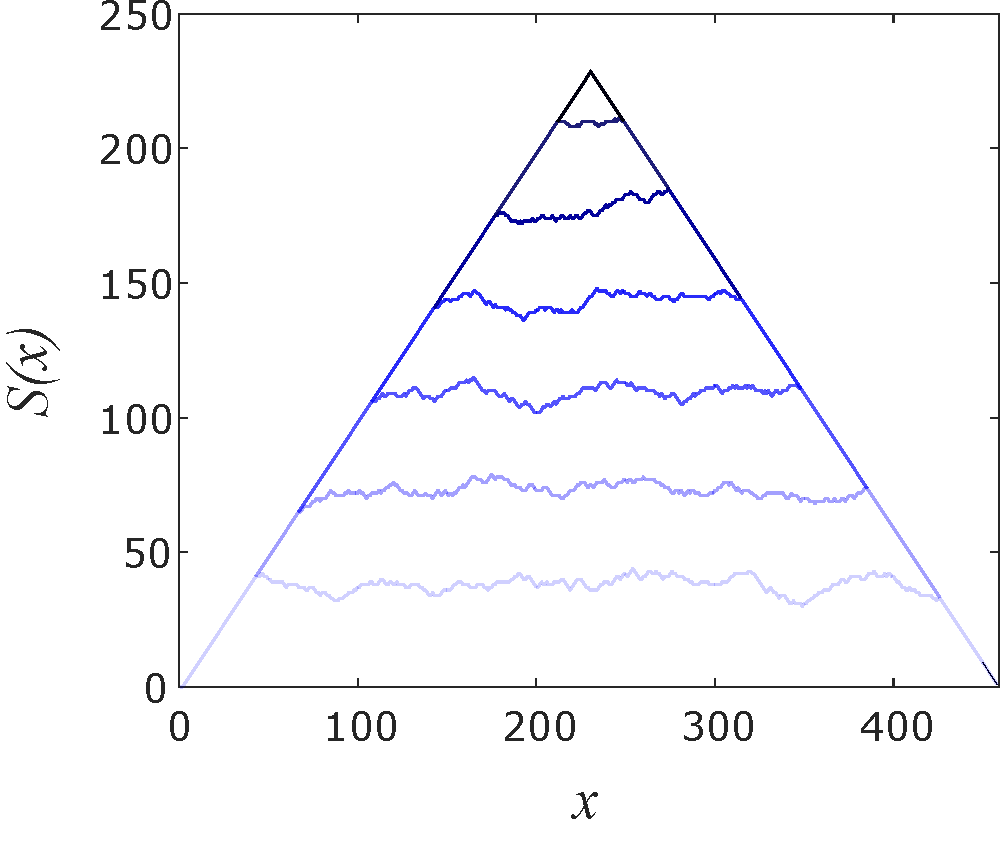
\includegraphics[width=.5\linewidth]{Tower}
	\caption{\textbf{Bitartite entanglement entropy at different times,} ($t = 340$, 690, 1024, 1365, 1707, 2048 and 4096). This data comes from a circuit model, but the behavior is believed to be general. Figure from~\cite{Nahum2017}.}
	\label{fig:Tower}
\end{figure}
The flat section has a constant growth rate $\pd{S(x,t)}{t}$ so the cusp position $y$ moves at a constant speed defined by the growth rate and the slope. Since the maximal slope is $\pd{S(x,t)}{x}=1$, this velocity is
\begin{align}
\pd{y}{t} = \pd{S}{t}\left(\pd{S}{x}\right)^{-1} = \pd{S}{x} = v_E.
\end{align}
This entanglement speed is equivalent to \_\_\_\_\_\_\_\_\_\_

References~\cite{Keyserlingk, Jonay, Nahum2017} discuss the speed of entanglement in brickwork models using related concepts called out of time order commutator (OTOC) and operator density. Reference~\cite{Zhou2017} quantifies the scrambling using the operator entanglement entropy opEE of the time evolution operator.
